% Document class and two-column conversion
\documentclass[twocolumn]{report}
% dimensions of paper and relative text positioning
\usepackage[a4paper,top=2cm,bottom=2cm,left=2cm,right=2cm]{geometry}
% math symbols
\usepackage{amsmath}
\usepackage{amssymb}
% package for including URLs
\usepackage{url}
% Required for including images
\usepackage{graphicx}
\usepackage{float} % Required for specifying the exact location of a figure

% enable writing in greek
\usepackage[greek,english]{babel}
\usepackage[utf8]{inputenc}

\setlength{\parindent}{0pt} % Removes all indentation from paragraphs

% Start of the document
\begin{document}

% Set the language to greek
\selectlanguage{greek}

% Title page
\title{\Huge \bfseries Τεχνικές Βελτιστοποίησης \\ \selectlanguage{english}Project 2024\selectlanguage{greek}} %\Huge and \bfseries are used to make the title bigger and bold
\author{Παπαδάκης Κωνσταντίνος Φώτιος\vspace{0.5cm} \\  ΑΕΜ:10371} % \vspace{0.5cm} is used to add some vertical space between the author and the AEM
\date{\today}
% prints the title, author and date on a separate page
\maketitle

% General introduction
\section*{Γενετικοί Αλγόριθμοι}
Οι γενετικοί αλγόριθμοι είναι μια κατηγορία αλγορίθμων βελτιστοποίησης οι
οποίοι εμπνέονται από τον μηχανισμό της εξέλιξης που συναντάμε στη φύση.
Ξεκινάμε με ένα πληθυσμό από διαφορετικές λύσεις του προβλήματος, συνήθως 
τυχαίες, και έπειτα, ύστερα από διάφορες τυχαίες μεταλλάξεις και διασταυρώσεις 
αυτών (γονείς), επιλέγουμε τις καταλληλότερες λύσεις για να διαμορφώσουμε 
την επόμενη γενιά (παιδιά).
\begin{figure}[H]
    \centering
    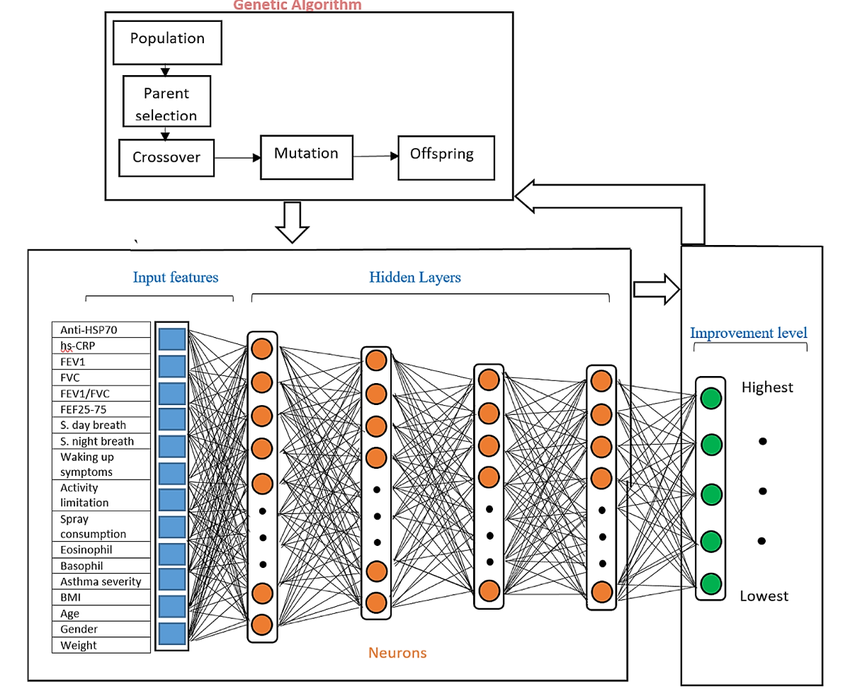
\includegraphics[width=0.4\textwidth]{media/genetic_algorithm.png}
    \caption{Γενετικός Αλγόριθμος}
\end{figure}

% Mathematical formulation
\section*{Θέμα 1\\Μαθηματική Διατύπωση}
Να δοθεί η μαθηματική διατύπωση του προβλήματος.
\subsection*{Λύση}
Από το πρόβλημα μας ζητείται να ελαχιστοποιήσουμε ως προς $x_i$ τον συνολικό
χρόνο διάσχισης του δικτύου:
\begin{figure}[H]
    \centering
    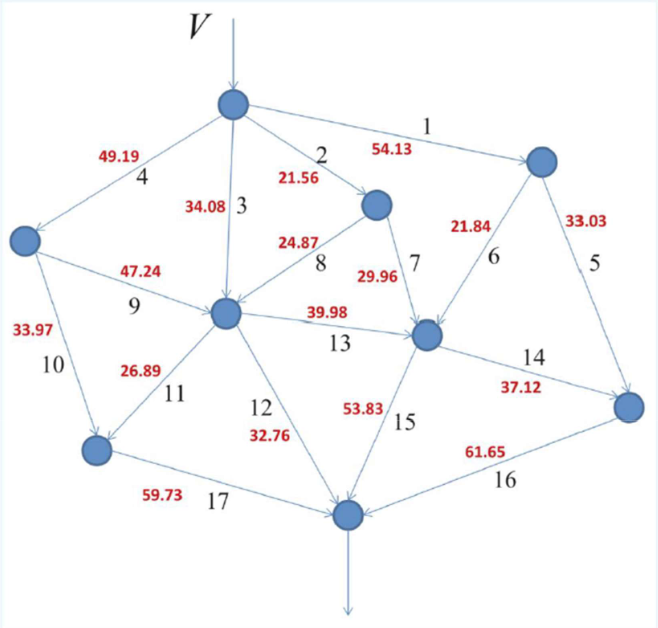
\includegraphics[width=0.4\textwidth]{media/network.png}
    \caption{Το οδικό δίκτυο}
\end{figure}

Η εξίσωση, που υπολογίζει τον χρόνο κίνησης στον δρόμο $i$ συναρτήσει του αριθμού 
των οχημάτων $x_i$, περιγράφεται από την εξίσωση:
$$f(x) = \sum_{i=1}^{17} \left( t_i + a_i \cdot \frac{x_i}{1 - \frac{x_i}{c_i}} \right)$$
Παρατηρούμε ότι καθώς το $t_i$ παραμένει σταθερό για τον εκάστοτε δρόμο, αρκεί 
να ελαχιστοποιήσουμε τη συνάρτηση:
$$g(x) = \sum_{i=1}^{17} a_i \cdot \frac{x_i}{1 - \frac{x_i}{c_i}}$$

Υπόψιν μας λαμβάνουμε τους εξής περιορισμούς:

\smallskip 

Εξισώσεις μεταξύ των $x_i$ οι οποίες προκύπτουν από την ισότητα εισόδου με εξόδου
των κόμβων:
\begin{itemize}
    \item $x_1 + x_2 + x_3 + x_4 = 100$
    \item $x_1 = x_5 + x_6$
    \item $x_2 = x_7 + x_8$
    \item $x_3 + x_8 + x_9 = x_{11} + x_{12}$
    \item $x_4 = x_9 + x_{10}$
    \item $x_6 + x_7 + x_{13} = x_{14} + x_{15}$
    \item $x_5 + x_{14} = x_{16}$
    \item $x_{10} + x_{11} = x_{17}$
    \item $x_{12} + x_{15} + x_{16} + x_{17} = 100$
\end{itemize}
Περιορισμοί στις τιμές που μπορεί να πάρει το κάθε $x_i$:
\begin{itemize}
    \item $0 \leq x_i \leq c_i$
\end{itemize}
Και τέλος για την αποφυγή της διαίρεσης με το μηδέν κατά τον υπολογισμό της $g(x)$:
$$g(x) = \sum_{i=1}^{17} a_i \cdot \frac{x_i}{1 - \frac{x_i}{c_i}+ \epsilon}$$
όπου $\epsilon = 10^{-6}$.

% Genetic Algorithm
\section*{Θέμα 2\\Γενετικός Αλγόριθμος}
Να υλοποιηθεί ένας γενετικός αλγόριθμος στο \selectlanguage{english}
Matlab\selectlanguage{greek} που να λύνει το πρόβλημα.
\subsection*{Λύση}
Υλοποιούμε τους περιορισμούς μεταξύ των $x_i$, λόγω της ισότητας εισόδου με εξόδου δικτύου,
περνώντας όλες τις μεταβλητές από την αριστερή πλευρά και αφήνοντας τους καθαρούς
αριθμούς από την απέναντι. Στην πράξη τα δεδομένα αυτά είναι πιο εύκολα διαχειρίσιμα 
υπό την μορφή δύο πινάκων:
\begin{itemize}
    \item $A_{eq}$: Πίνακας κάθε γραμμή του οποίου περιέχει τα $x_i$ της εκάστοτε 
    εξίσωσης (αριστερή πλευρά)
    \item $b_{eq}$: Πίνακας που περιέχει τα καθαρά νούμερα των εξισώσεων ισότητας 
    (δεξιά πλευρά)
\end{itemize}
Έπειτα αφού δημιουργήσουμε τους υπόλοιπους απλούς περιορισμούς που αναφέραμε και στην 
μαθηματική διατύπωση του προβλήματος, ορίζουμε τις ρυθμίσεις του γενετικού μας αλγορίθμου:
\begin{itemize}
    \item \selectlanguage{english}\textbf{CreationFcn:}\selectlanguage{greek} 
    Συγκεκριμενοποιούμε τον τρόπο δημιουργίας του αρχικού πληθυσμού. 
    \begin{itemize}    
        \item \selectlanguage{english}@gacreationlinearfeasible\selectlanguage{greek}
        Ελέγχει ότι οι τιμές του αρχικού πληθυσμού είναι εντός των γραμμικών περιορισμών
        που θέτουμε στους πίνακες $A_{eq}$ και $b_{eq}$.
    \end{itemize}

    \item \selectlanguage{english}\textbf{CrossoverFcn:}\selectlanguage{greek} 
    Επιλέγουμε τον τρόπο διασταύρωσης των γονιδίων από τους γονείς.
    \begin{itemize}
        \item \selectlanguage{english}@crossoverintermediate\selectlanguage{greek}
        Τα παιδιά προκύπτουν από την εξής σχέση: $$ O = P_1 + \alpha \cdot (P_2 - P_1) $$,
        όπου $O$ είναι το παιδί, $P_1$ και $P_2$ οι γονείς και $\alpha$ ένας τυχαίος αριθμός
        μεταξύ 0 και 1.
    \end{itemize}

    \item \selectlanguage{english}\textbf{SelectionFcn:}\selectlanguage{greek} 
    Επιλέγουμε τον τρόπο επιλογής των γονέων.
    \begin{itemize}
        \item \selectlanguage{english}@selectionstochunif\selectlanguage{greek}
        Εφαρμόζει στοχαστική ομοιόμορφη επιλογή γονέων.
    \end{itemize}

    \item \selectlanguage{english}\textbf{MutationFcn:}\selectlanguage{greek}
    Επιλέγουμε τον τρόπο μετάλλαξης των γονιδίων.
    \begin{itemize}
        \item \selectlanguage{english}@mutationadaptfeasible\selectlanguage{greek}
        Εξακριβώνει ότι οι μεταλλάξεις υπακούν στους περιορισμούς που έχουμε θέσει.
    \end{itemize}

    \item \selectlanguage{english}\textbf{Display:}\selectlanguage{greek}
    Επιλέγουμε τι πληροφορία προβάλλεται στη κονσόλα κατά την εκτέλεση του αλγορίθμου.
    \begin{itemize}
        \item \selectlanguage{english}iter:\selectlanguage{greek}
        Τυπώνεται η αναλυτική εξέλιξη του αλγορίθμου κάθε γενιά.
    \end{itemize}

    \item \selectlanguage{english}\textbf{MaxGenerations:}\selectlanguage{greek}
    Ορίζουμε τον μέγιστο αριθμό γενεών που θα εκτελεστεί ο αλγόριθμος.

    \item \selectlanguage{english}\textbf{PopulationSize:}\selectlanguage{greek}
    Ορίζουμε το μέγεθος του πληθυσμού που συμμετέχει στον γενετικό αλγόριθμο.
\end{itemize}
Εκτελώντας το πρόγραμμα καταγράφουμε παράλληλα και τα $fitness levels$ ή αλλιώς την
τιμή της συνάρτησης $g(x)$ για κάθε γενιά. Το παραγόμενο γράφημα είναι το εξής:
\begin{figure}[H]
    \centering
    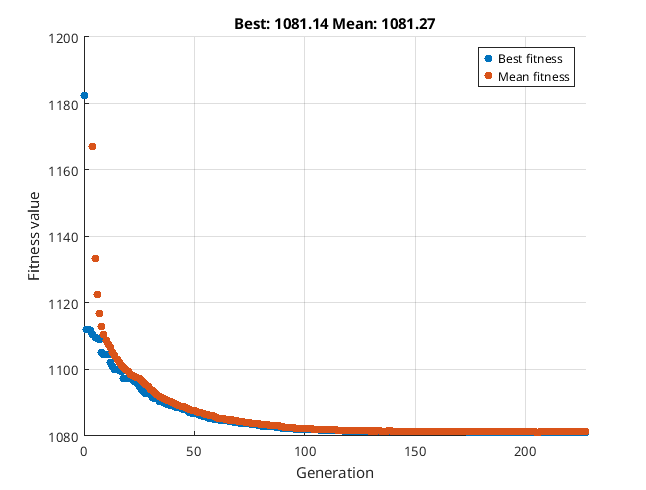
\includegraphics[width=0.4\textwidth]{media/plotV.png}
    \caption{Τιμές της συνάρτησης $g(x)$ ανά γενιά}
\end{figure}
Αν και βρίσκουμε το ελάχιστο της συνάρτησης $g(x)$, η βέλτιστη λύση περιλαμβάνει μέσα και 
τις σταθερές των δρόμων. Οπότε στο τελικό αποτέλεσμα πρέπει να προστεθεί:
$$t_{sum} = \sum_{i=1}^{17} t_i$$

% Alternate 
\section*{Θέμα 3\\Μεταβαλλόμενο \selectlanguage{english}V\selectlanguage{greek}}
Θεωρήστε ότι ο ρυθμός εισερχομένων οχημάτων $V$ μπορεί να μεταβάλλεται μέχρι 
$\pm 15\%$ της αρχικής του τιμής. Να επιλυθεί το πρόβλημα εκ νέου με 
την ίδια μεθοδολογία βελτιστοποίησης. 
\subsection*{Λύση}
Διατηρώντας τον ίδιο αλγόριθμο βελτιστοποίησης, προσθέτουμε τα δύο ακραία ενδεχόμενα 
που προκύπτουν όταν το $V$ μεταβάλλεται κατά $\pm 15\%$ της αρχικής του τιμής.
Οι νέες γραφικές παραστάσεις που προκύπτουν είναι οι εξής:
\begin{figure}[H]
    \centering
    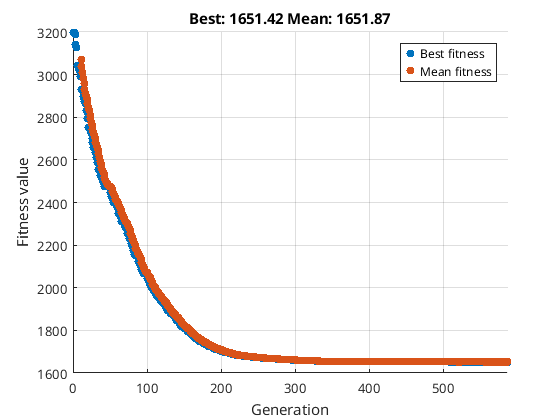
\includegraphics[width=0.4\textwidth]{media/plotVmax.png}
    \caption{Για $Vmax = 1.15V$}
\end{figure}
\begin{figure}[H]
    \centering
    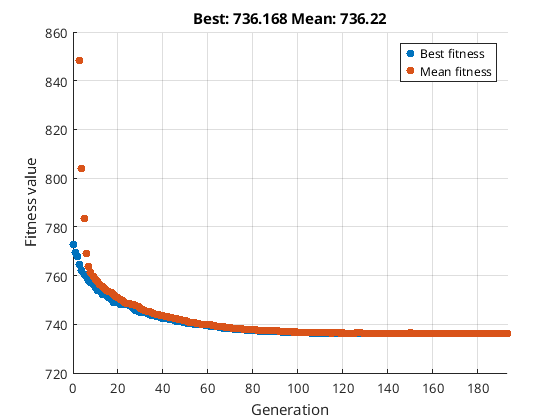
\includegraphics[width=0.4\textwidth]{media/plotVmin.png}
    \caption{Για $Vmin = 0.85V$}
\end{figure}
Παρατηρούμε ότι για λιγότερη κίνηση εισόδου ο χρόνος διάσχισης του δικτύου είναι
μικρότερος και αντίστοιχα για περισσότερη κίνηση εισόδου ο χρόνος διάσχισης είναι
μεγαλύτερος. Αυτό ήταν αναμενόμενο καθώς πέφτουν ή ανεβαίνουν αντίστοιχα, ανάλογα
την περίπτωση, οι τιμές των μεταβλητών $x_i$.

Τέλος, για την καλύτερη οπτικοποίηση της εκτέλεσης του γενετικού αλγορίθμου προσθέτουμε
την ρύθμιση $@gaplotbestf$ στη συνάρτηση $ga()$ και το επιπλέον στάδιο της επαλήθευσης 
εντός της συνάρτησης $fitnessFunction()$ το οποίο μας επιτρέπει να αποφεύγουμε
μεταλλάξεις οι οποίες οδηγούν σε αναλογίες $\frac{x_i}{c_i}$ που αυξάνουν υπερβολικά πολύ το 
παραγόμενο καθε γενιά αποτέλεσμά μας: $T$. 

% Comments
\section*{Παρουσίαση Αποτελεσμάτων}
Βάσει των παραπάνω μεθόδων συνθέτουμε ένα τελευταίο αρχείο $Matlab$ το οποίο παίρνει
διάφορες τιμές της μεταβλητής $V$ και δημιουργεί τα αντίστοιχα γραφήματα των τελικών
$x_i$ (βλ. Σχήμα \ref{fig:optimalXplot}) και $Τ$ (βλ. Σχήμα \ref{fig:optimalTplot})
για κάθε τιμή της $V$. Μπορούμε να δούμε ότι ο συνολικός χρόνος $T$ αυξάνεται σχεδόν 
γραμμικά όσο αυξάνουμε την κίνηση εισόδου $V$. Παράλληλα οι τιμές $x_i$ είναι και αυτές 
σε γενικές γραμμές ανάλογες της κίνησης εισόδου $V$ με τις εξής εξαιρέσεις:
\begin{itemize}
    \item Η ακμή $x_8$
    \item Η ακμή $x_{10}$
    \item Η ακμή $x_{13}$
    \item Η ακμή $x_{15}$
\end{itemize}
Οι ακμές $8, 10$ και $13$ παραμένουν σταθερές για όλες τις τιμές της $V$ ενώ η ακμή
$15$ δεν εμφανίζει κάποια συγκεκριμένη τάση. Τα γραφήματα βρίσκονται στην επόμενη σελίδα
για την ευκολία του αναγνώστη.

\onecolumn
\begin{figure}[H]
    \centering
    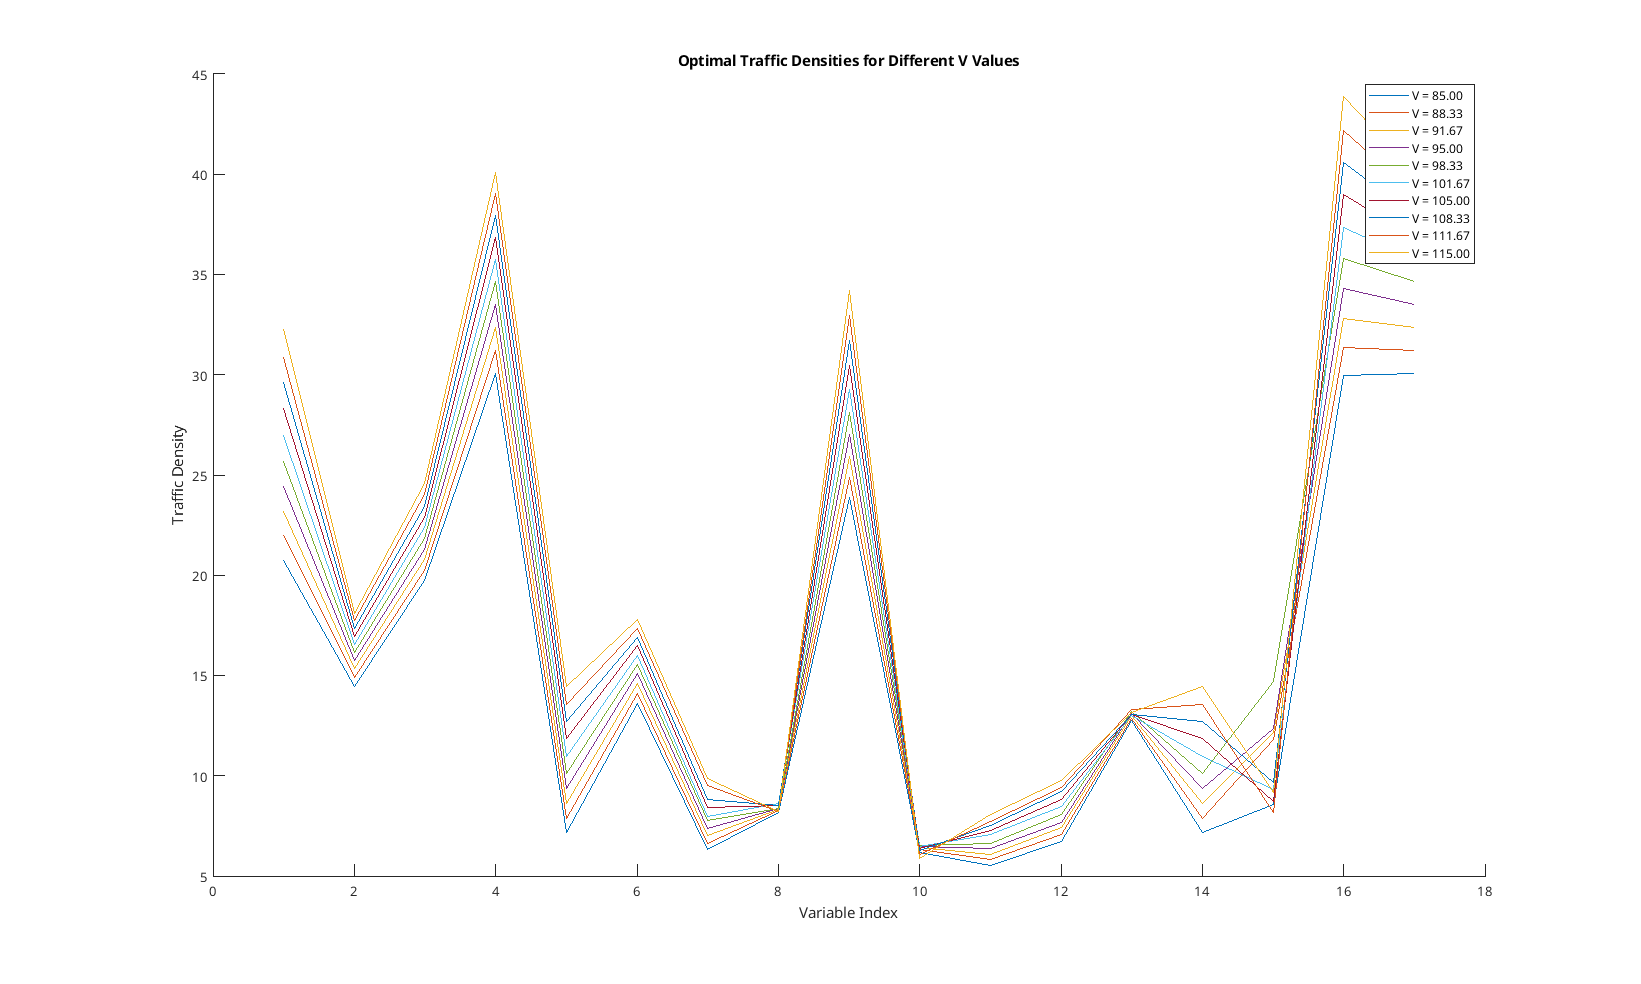
\includegraphics[width=1\textwidth]{media/optimalXplot.png}
    \caption{Βέλτιστα $x_i$ για διάφορες τιμές της $V$}
    \label{fig:optimalXplot}
\end{figure}
\begin{figure}[H]
    \centering
    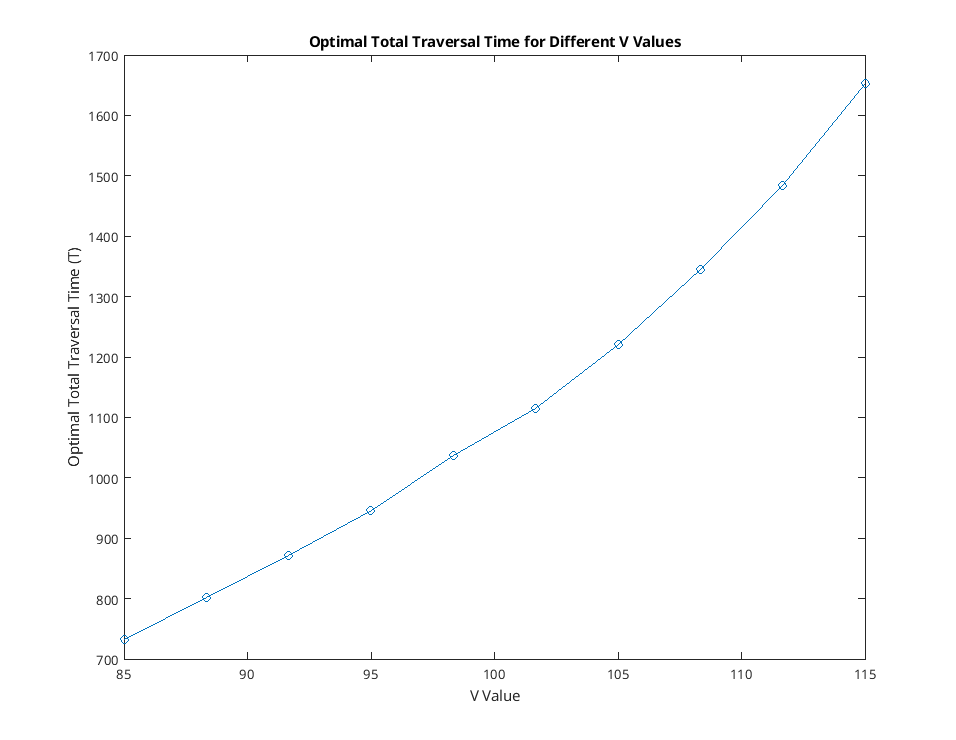
\includegraphics[width=0.8\textwidth]{media/optimalTplot.png}
    \caption{Βέλτιστα $T$ για διάφορες τιμές της $V$}
    \label{fig:optimalTplot}
\end{figure}


% End of the document
\end{document}